% THIS IS SIGPROC-SP.TEX - VERSION 3.1
% WORKS WITH V3.2SP OF ACM_PROC_ARTICLE-SP.CLS
% APRIL 2009
%
% It is an example file showing how to use the 'acm_proc_article-sp.cls' V3.2SP
% LaTeX2e document class file for Conference Proceedings submissions.
% ----------------------------------------------------------------------------------------------------------------
% This .tex file (and associated .cls V3.2SP) *DOES NOT* produce:
%       1) The Permission Statement
%       2) The Conference (location) Info information
%       3) The Copyright Line with ACM data
%       4) Page numbering
% ---------------------------------------------------------------------------------------------------------------
% It is an example which *does* use the .bib file (from which the .bbl file
% is produced).
% REMEMBER HOWEVER: After having produced the .bbl file,
% and prior to final submission,
% you need to 'insert'  your .bbl file into your source .tex file so as to provide
% ONE 'self-contained' source file.
%
% Questions regarding SIGS should be sent to
% Adrienne Griscti ---> griscti@acm.org
%
% Questions/suggestions regarding the guidelines, .tex and .cls files, etc. to
% Gerald Murray ---> murray@hq.acm.org
%
% For tracking purposes - this is V3.1SP - APRIL 2009

\documentclass{acm_proc_article-sp}
\usepackage{mathtools}

\begin{document}

\title{Development of a control logic for\\Mixed-Reality-Robot mrShark}
\subtitle{Considering up-to-date small batch productions tecniques}
%
% You need the command \numberofauthors to handle the 'placement
% and alignment' of the authors beneath the title.
%
% For aesthetic reasons, we recommend 'three authors at a time'
% i.e. three 'name/affiliation blocks' be placed beneath the title.
%
% NOTE: You are NOT restricted in how many 'rows' of
% "name/affiliations" may appear. We just ask that you restrict
% the number of 'columns' to three.
%
% Because of the available 'opening page real-estate'
% we ask you to refrain from putting more than six authors
% (two rows with three columns) beneath the article title.
% More than six makes the first-page appear very cluttered indeed.
%
% Use the \alignauthor commands to handle the names
% and affiliations for an 'aesthetic maximum' of six authors.
% Add names, affiliations, addresses for
% the seventh etc. author(s) as the argument for the
% \additionalauthors command.
% These 'additional authors' will be output/set for you
% without further effort on your part as the last section in
% the body of your article BEFORE References or any Appendices.

\numberofauthors{1} %  in this sample file, there are a *total*
% of EIGHT authors. SIX appear on the 'first-page' (for formatting
% reasons) and the remaining two appear in the \additionalauthors section.
%
\author{
% You can go ahead and credit any number of authors here,
% e.g. one 'row of three' or two rows (consisting of one row of three
% and a second row of one, two or three).
%
% The command \alignauthor (no curly braces needed) should
% precede each author name, affiliation/snail-mail address and
% e-mail address. Additionally, tag each line of
% affiliation/address with \affaddr, and tag the
% e-mail address with \email.
%
% 1st. author
\alignauthor
Hannes Eilers\\
       \affaddr{University of Applied Sciences Kiel}\\
       \affaddr{24149 Kiel}\\
       \affaddr{Schleswig-Holstein, Germany}\\
       \email{mail@hannes-eilers.de}
% 2nd. author
% 3rd. author
% use '\and' if you need 'another row' of author names
% 4th. author
% 5th. author
% 6th. authorom
}
% There's nothing stopping you putting the seventh, eighth, etc.
% author on the opening page (as the 'third row') but we ask,
% for aesthetic reasons that you place these 'additional authors'
% in the \additional authors block, viz.
\additionalauthors{}
\date{04 December 2014}
% Just remember to make sure that the TOTAL number of authors
% is the number that will appear on the first page PLUS the
% number that will appear in the \additionalauthors section.

\maketitle
\begin{abstract}
The Mixed-Reality is a robot soccer league, using a half-virtual system for
developing an artifical intelligence (AI) that's playing soccer. Already in use
robots for the system arent't available any more, so a re-development was
necessary. This paper summarizes the result from a bachelor thesis developing
the control logic for a new Mixed-Reality-Robot. It includes a micro-controller
driven control logic and consideres up-to-date small batch production
techniques for choosing proper electronic components and electronic layout.
\end{abstract}

% A category with the (minimum) three required fields
%\category{H.4}{Information Systems Applications}{Miscellaneous}
%A category including the fourth, optional field follows...
%\category{D.2.8}{Software Engineering}{Metrics}[complexity measures,
% performance measures]

%\terms{Theory}

\keywords{Micro-Robot, Mixed-Reality, Control logic, Printed-Circuit-Board, Small batch
production techniques} % NOT required for Proceedings

\section{Introduction}
The Mixed-Reality (MR) bases on a half-virtual robot system for developing AIs
on a soccer scenario. For that small robots with dimension about
$3cm^{2}$ \cite{northernstars:mrshark}, are driving on a screen with simulated
soccer field and simulated soccer ball. One or multiple cameras are tracking the robots using marker codes on their top side. The tracked position is projected
into the simulated soccer field, wich is used for an external agent program that
can remote control the robot using an infrared transmitter system. The advantages of the system are a hardware-independent
framework for AI programming and reduced hardware problems normally occuring
with full reality robot-system, like orientation problems, autonomous working
problems or limited on-robot resources\cite{northernstars:mr-system}.
\newline
\newline
Mixed-Reality robots used in the past where developed and manufactured by the
CITIZEN company\cite{rtlions:faq}. Currently CITIZEN is no more producing new
robots and is not planning to do this in future. These orginal CITIZEN-Robots are titled as old
bots and new developments are titled as new bots. Due to problems with
unavailable components of the old robots and difficult maintance of the
components, a re-development was necessary. That should consider long
avilability of components, easy maintance and cheap small batch production. Also
compatibility of new systems with the old system are needed to enable easy
changing to a new system. A bachelor thesis at the University of Applied
Sciences Kiel worked on this and developed an electronic control circuit with
printed-circuit-board (pcb) for a new bot called mrShark.

% ---------------------------------------------------------------------
% INDUSTRIAL PCB BATCH PRODUCTION TECHNIQURES
% ---------------------------------------------------------------------
\section{Industrial pcb batch\\ production techniques}
For re-development of a MR-Robot it was important to consider production
techniques to select cost-efficient and highly available components as well as
generating a proper producable pcb layout. In general industrial batch
production of pcbs is divided into two steps, the production of the pcb itself
and the assembly of the electronic components. For the first step the
pcb layout mainly needs to consider dimension and spacings of circuit paths,
where in the seconds step the electronic components playing a major role. They
are influencing the costs for assembling the pcb because of higher programming
costs of the assembly machine for a higher components diversity or using
different assembling techniques as surface mounted devices (SMD) \cite{sautter:88} and
thorugh hole technology (THT) \cite{scheel:97}. Also placeing only a few components on one
side (layer) of the pcb is inefficient due to extra costs for programming the assembly
machine for assembling the second side. The total number of components is also
important due to limitations of the maximum capacity of components storage at
one assembly machine. All this needs to be considered while choosing an
electronic component \cite{eilers:13}.

% ---------------------------------------------------------------------
% REQUIREMENTS FOR mrShark
% ---------------------------------------------------------------------
\section{Requirements for mrShark}
From the problems of the old bots and the techniques applied during industrial
batch production the following requirements are arising \cite{eilers:13}:
\begin{itemize}
  \item Cheap production
  \item Highly available electronic components/devices
  \item Simple programming
  \item Simple extending
  \item Long runtime
  \item Autonomous power supply
  \item Compatibility with existing system
  \item Measurement of relevant system voltages and currents
  \item Optimization in view of industrial small batch productions
\end{itemize}

\subsection{Limitations}
Due to backward compatibility the new system has some limitations as following
\cite{eilers:13}:
\begin{itemize}
  \item PCB dimension max. 31,0x26,0mm (right angle) with 45 degree phase on
  all four edges
  \item Using 2 GM15 dc motors
  \item Remote control via 115,2kBit/s infrared signal
 \end{itemize}

% ---------------------------------------------------------------------
% CONTROL LOGIC
% ---------------------------------------------------------------------
\section{Control logic}
The control logic of the mrShark robot is used to recieve remote infrared data,
to control the robots motors and to show it's current state. The control logic
is explained in details below.

\section{Concept}
The concept of realising a electronic ciruit was a mircocontroller based
solution with some external integrated circuits (IC) (see figure \ref{fig:concept}) for
controlling the motor voltage and current as well as an infrared to serial
decoder for decoding remote infrared data and some integrated analog to digital
converters (ADC) for mesearuring the relevant voltage. Rgb leds are used to
light up the robots case and to show it's current state. Finally an
interface should be used to extend the system with additional electronics.

\begin{figure}
\centering
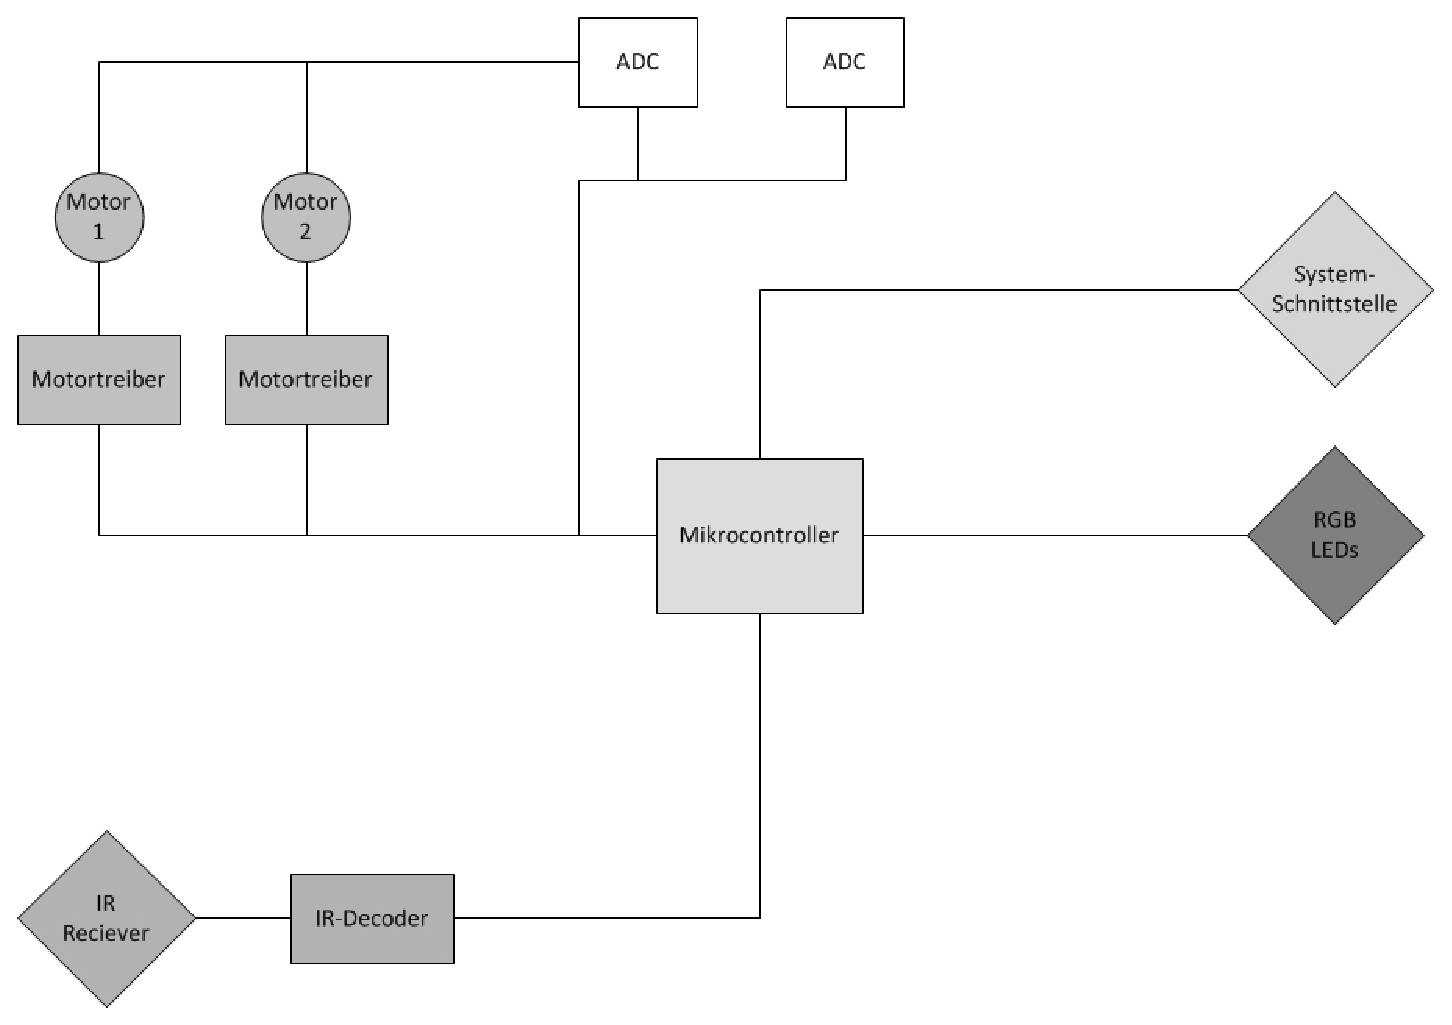
\epsfig{file=img/concept.eps, width=3.3in}
\caption{Mixed-Reality robot mrShark electronic circuit concept.}
\label{fig:concept}
\end{figure}

\subsection{Power supply}
The power supply should be able to enable a long autonomous runtime without
recharging. For that two lithium-polymer (LiPo) rechargable batteries are used
in parrellel mode. With that the supply voltage ist between 4.1V and 3.3V\cite{eilers:13}.
The rechargable LiPo-batteries offering a long runtime without any need to replace
them. They have also small dimensions and enabling a high capacity in parallel mode.

\subsection{System interface}
The system interface uses a pin-header in the middle of the robot's pcb to
prodive internal voltages (like battery voltages) and communication data for
external electronics that could get mounted above the control logic's pcb.

\subsection{Components}
As central processing unit an AVR ATmega168 microntroler with 16MB program flash
is used. The microntroler provides enough computing power and program data ram
for analysing incoming remote data streams and measured data. On the other hand
the device integrades often used peripherals with a minimum of power consumption
(see figure \ref{fig:avrsupplycurrent}). The ATmega168 can get replaced with
the ATmega48 or ATmega88 devices with 4MB and 8MB program flash. These optional
devices are cheaper but offer less program memory.

The mrShark control logic also includes an infrared to serial decoder and two
motor drivers, two Twisted-Wire-Interface-Bus (TWI-Bus) ADC are used, as well
as an TWI-Bus Switch to switch between internal and external TWI master devices
in case of using many robots connected together.

The control logic uses a status led and four rgb-leds to illuminate the robot's
case and for providing visual information about the robot's state.

\begin{figure}
\centering
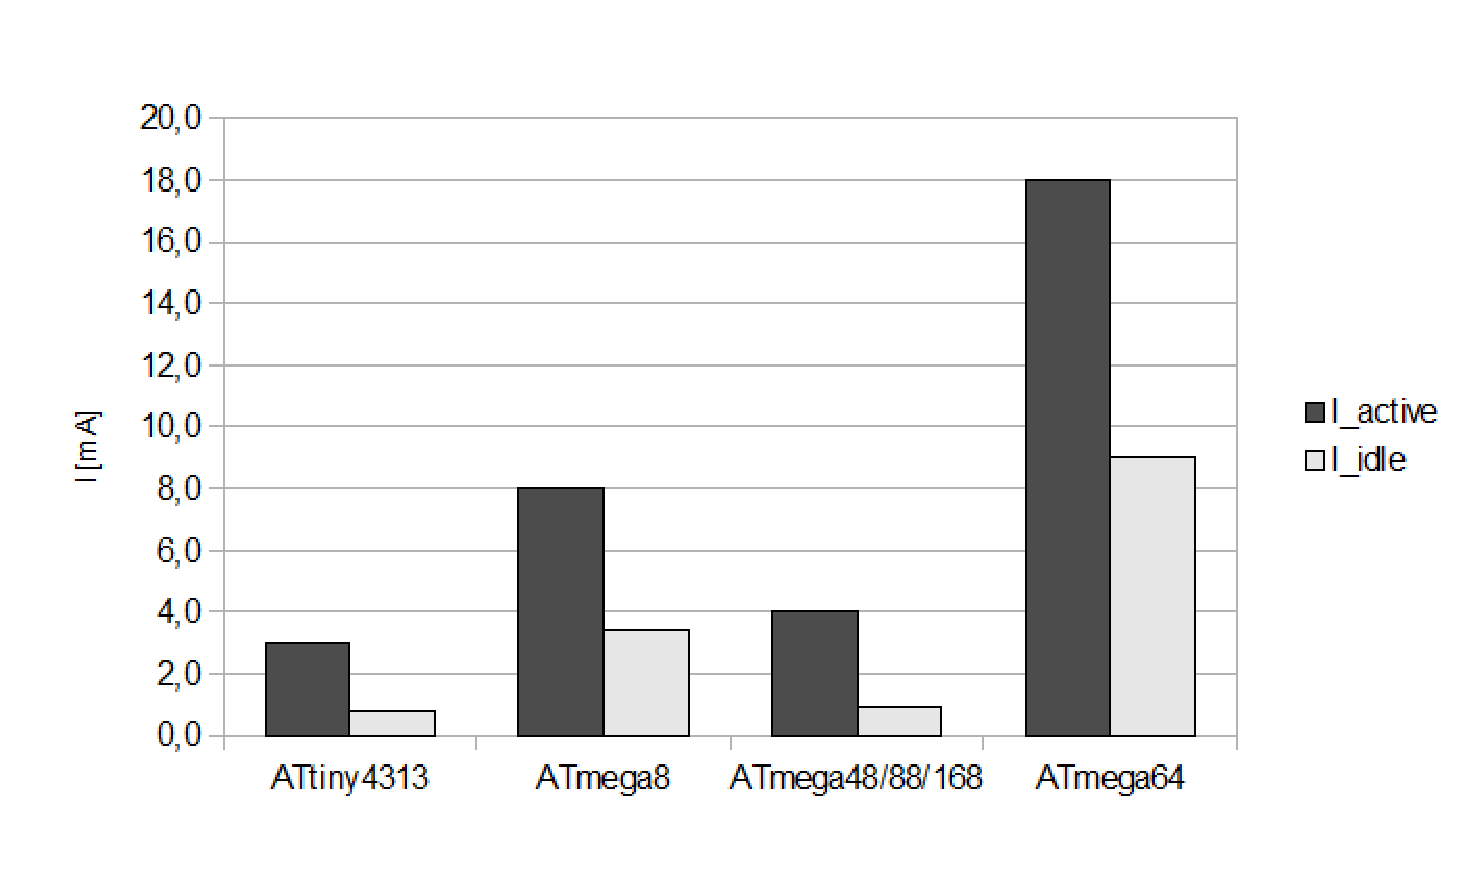
\epsfig{file=img/avr-supply-current-sw.eps, width=3.3in}
\caption{Supply current [mA] of different AVR microcontroler devices in active
and idle state.}
\label{fig:avrsupplycurrent}
\end{figure}


% ---------------------------------------------------------------------
% VALIDATION
% ---------------------------------------------------------------------
\section{Evaluation}
The electronic components used and the layout of the
control logics pcb are selected to  provide a product life-cycle as long as
possible, as well as small batch production costs. For that the worldwide
availability of components, the diversity of component types used and the layout
arrangement of components at the pcb are evaluated. Not rated are state of the
art components like often used resistors and capacitors, because often they are
in-stock products of pcb production companies. The evaluation uses point in
range of 0 to 100 to rate every evaluation item on a fictive production of 150
pcbs \cite{eilers:13}.

For the component availibility the products available at the worldwide
distrubutor Farnell was analysed at august 2013. For that the needed number of
components {n} and the available number of components {k} were used. A
multiplicator {m} indicates the art of availibilty (see equation
\ref{eq:component-availibility}).
For components in Farnell's EU stock {m} is 1.0, for components only available
in Farnell's US stock it is 0.75, if components are only available from other
distrubutor it is 0.5, for components only available from producer it is 0.25 and 0.0 for unavailable
products\cite{eilers:13}.

\begin{equation}
\label{eq:component-availibility}
P_{1} = \frac{k}{n}*m*100 \text{points}
\end{equation}

For the 17 most important components, an average 91 of 100 points is reached.
Two components are only available from other distributors than Farnell and one
component has the be ordered directly from producer (see figure
\ref{fig:evavailibility}).

\begin{figure}
\centering
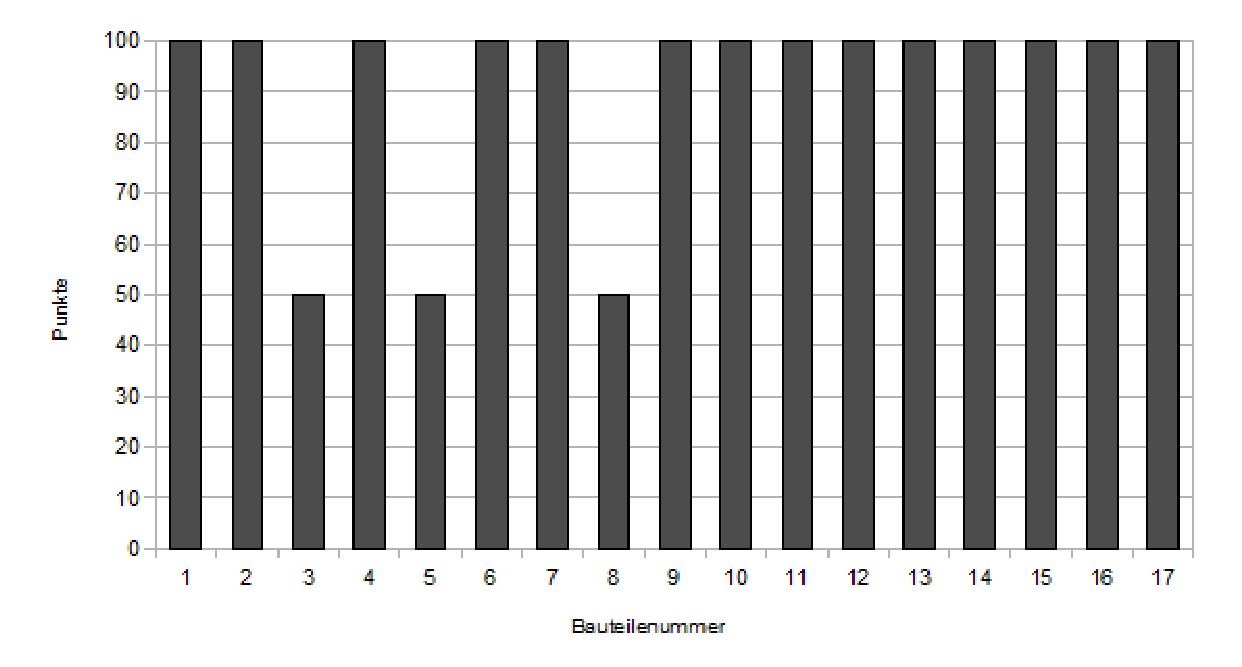
\epsfig{file=img/evaluation-availibility.eps, width=3.3in}
\caption{Evaluation points for most important control logic components (by
number).}
\label{fig:evavailibility}
\end{figure}

For component diversity a quotient of different component types {v} and total
number of components {n} is used (see equation \ref{eq:component-diversity}). So
less diversity is rated bettern in case of lower machine programming costs
during production.

\begin{equation}
\label{eq:component-diversity}
P_{2} = (1 - \frac{v}{n}) * 100 \text{points}
\end{equation}

For 26 different and total 66 components the mrShark control logic pcb reaches
an average 61 of 100 points \cite{eilers:13}.

For the evaluation of the pcb's layout the number of components on each side of
the 2-layer pcb, as well as the number of different orientations are used (see
equation \ref{eq:component-layout}). Where $n_{MINOR}$ is the number of components on the pcb
side with the least number of these components and $n_{MAJOR}$ the number of
components on the other side. The multiplicator {m} is 1.0 if all
components of one type having the same orientation. For every additional
orientation it is decreased by 0.25.

\begin{equation}
\label{eq:component-layout}
P_{3} = \frac{n_{MINOR}}{n_{MAJOR}}*m*100 \text{points}
\end{equation}

The average number of points of the pcb's components layout is 87 of 100 points,
where 5 from total 26 component types have two different orientations and 3
component types have more than two different orientations \cite{eilers:13}.

The average of all three evaluation aspects, availibilty ($P_{1}$), diversity
($P_{2}$) and layout ($P_{3}$) is 80 of 100 points (see equation
\ref{eq:evaluation-total}) \cite{eilers:13}.

\begin{equation}
\label{eq:evaluation-total}
P = \frac{ P_{1} + P_{2} + P_{3} }{ 300 \text{points} } * 100 \text{points}
\end{equation}

% ---------------------------------------------------------------------
% CONCLUSION
% ---------------------------------------------------------------------
\section{Conclusion}
The developed control logic for the new Mixed-Reality robot mrShark offers
control of two DC-motors via infrared interface. The choosen micocontroller AVR
ATmega168 provides enough computing power and memory storage for complex
programs. The additional periphery offers possibilities to control different
volatges and a system interface provides the possibility to extend the system
with additional electronic circuits. The selected components used for the pcb and
their layout on the pcb are analysed and evaluated for small batch productions
with an overall good result. With these features the mrShark can be used as
replacement system for old Mixed-Relaity robots.

%\end{document}  % This is where a 'short' article might terminate

%
% The following two commands are all you need in the
% initial runs of your .tex file to
% produce the bibliography for the citations in your paper.
\bibliographystyle{abbrv}
\bibliography{references}  % sigproc.bib is the name of the Bibliography in
% this case You must have a proper ".bib" file
%  and remember to run:
% latex bibtex latex latex
% to resolve all references
%
% ACM needs 'a single self-contained file'!
% That's all folks!
\end{document}
